% !TEX encoding = UTF-8
% !TEX TS-program = pdflatex
% !TEX root = ../tesi.tex

%**************************************************************
\chapter{Architettura generale ed analisi composizione container}
\label{cap:analisi-progetto-container}
%**************************************************************

\intro{Breve introduzione al capitolo}\\
In questo capitolo si esporrà l'architettura generale del progetto implementata in Azienda, fornendo un'analisi dettagliata sulla composizione di ogni Dockerfile relativo ad ogni container. Infine, verrà esposto il meccanismo di costruzione automatizzato di una sandbox applicativa.

\section{Architettura generale}
%TODO: immagine architettura generale e relativa spiegazione anche del concetto di sandbox applicativa di HDA, con relativa possibilità di aggiornamento ed avanzamento di versione.

\section{Composizione container}
Come già precedentemente spiegato in questo documento, un container è un'unità atomica contenente un applicativo con le relative dipendenze atte al suo corretto funzionamento. Ogni container, ad esclusione del container "nginxcontainer" si basa su un'immagine del sistema operativo "Windows ServerCore IIS".
La composizione di un container può essere più facilmente espressa tramite la seguente immagine:
%TODO: immagine container + IIS + app
Per necessità progettuali che saranno descritte nel corso di questa relazione è stata necessaria la costruzione di sei diversi container. Di seguito è fornita al lettore una panoramica dettagliata sulla composizione di ognuno dei singoli.\\

\subsection{Container "hdaprepcontainer":}

\begin{namespacedesc}
	\classdesc{S.O./immagine di base} {Windows Servercore IIS}
	\classdesc{Immagine in output} {hdaprepimg}
	\classdesc{Descrizione} {Lo scopo del seguente container è quello di installare una istanza di HDA all'interno di esso, popolando quindi il volume-mapping condiviso con l'host con tutti i file di HDA con i relativi permessi dell'utenza di IIS impostati in automatico dal processo di installazione di HDA lanciato dall'eseguibile "update.exe".
Una volta terminata l'installazione, il container terminerà automaticamente la sua esecuzione. Per lanciare una istanza di HDA containerizzata bisognerà quindi eseguire il successivo container "hdabasecontainer" spiegato immediatamente.}
\end{namespacedesc}
\subsection{Container "hdabasecontainer"}

\begin{namespacedesc}
	\classdesc{S.O./immagine di base} {hdaprepimg}
	\classdesc{Immagine in output}{hdabaseimg}
	\classdesc{Descrizione} {Lo scopo del seguente container è quello di avviare, ed eventualmente re-installare, una istanza di HDA con i relativi servizi. Una volta fatto quanto specificato, a differenza del container hdaprepcontainer, questo non interromperà la sua esecuzione, ma rimarrà attivo per permettere ad utenti esterni di usufruire del programma HDA collegandosi alla web-interface propria dell'istanza di HDA in esecuzione. In aggiunta a questa istanza, è presente una installazione dell'applicativo "Telegraf", atto al monitoraggio in real time dell'istanza di HDA in esecuzione. 
Per favorire uno scambio di dati tra host questo container si interfaccia direttamente con due volume-mapping condivisi con l'host:
\begin{itemize}
	\item \textbf{hdashared}: è il volume-mapping che espone la cartella "App\_Data" del programma HDA. Questo volume-mapping permette all'installatore di esportare od importare degli overrides applicativi per delle customizzazioni specifiche di ogni cliente create ad-hoc dal team di sviluppo sulla base delle esigenze del cliente stesso.
	\item \textbf{lokishared}: è il volume-mapping che espone tutti i log applicativi dell'istanza di HDA, come ad esempio \textit{hda\_log.txt}, \textit{error\_log.txt}, \textit{wsc4\_log.txt}.. al container "lokicontainer" atto al monitoraggio dell'istanza di HDA presente in questo container.
\end{itemize}
Questo container dipende (eredita) il filesystem  ed i relativi permessi precedentemente configurati dal container "hdaprepcontainer".}
\end{namespacedesc}

\subsection{Container "hdadbupdatercontainer"}
\begin{namespacedesc}
	\classdesc{S.O./immagine di base} {hdabaseimg}
	\classdesc{Immagine in output}{hdabasedbimg}
	\classdesc{Descrizione} {Lo scopo del seguente container è quello di eseguire un aggiornamento del database di HDA manualmente creato all'interno di uno specifico server \textbf{MS-SQL}. I parametri di connessione al database pre-esistente di HDA sono nel template-file "istance.json" presente nel pacchetto di installazione di HDA fornito.
Il presente container non ha associato alcun indirizzo IP o scheda di rete virtuale, in quanto l'utente non ha la necessità di interfacciarcisi durante la sua esecuzione e può, inoltre, essere eseguito indipendentemente da qualsiasi altro container in esecuzione sullo stesso host.
La versione di HDA presente nel container "hdaprepcontainer", e di conseguenza nel container "hdabasecontainer", deve essere compatibile con la versione del database installato tramite questo container. Il controllo di versione non è automatizzato, e lo dovrà quindi fare il tecnico installatore manualmente. La tabella informativa relativamente alla compatibilità tra versioni di HDA e database è presente all'interno del file Onenote aziendale.  
}
\end{namespacedesc}

\subsection{Container "lokicontainer"}
\begin{namespacedesc}
	\classdesc{S.O./immagine di base} {Windows Servercore IIS}
	\classdesc{Immagine in output}{lokiimg}
	\classdesc{Descrizione} {Lo scopo del seguente container è quello di eseguire una istanza del programma "Loki" atto al monitoraggio dei servizi di HDA. Il presente container preleva i dati popolati dall'istanza di HDA in esecuzione nel container "hdabasecontainer" nel volume mapping "lokishared"  ad esso collegato, per inviarli direttamente al container "promtailcontainer".}
\end{namespacedesc}

\subsection{Container "promtailcontainer"}
\begin{namespacedesc}
	\classdesc{S.O./immagine di base} {Windows Servercore IIS}
	\classdesc{Immagine in output}{promtailimg}
	\classdesc{Descrizione} {Lo scopo del seguente container è quello di eseguire una istanza del programma "Promtail" atto al monitoraggio dei servizi di HDA in esecuzione sul container "hdabasecontainer". Il seguente container espone i log collezionati dal container "lokicontainer" su una specifica porta precedentemente configurata da apposito file di configurazione "\textit{promtail-local-config.yml"} per permettere all'applicativo "Grafana", in esecuzione su un altro \textit{host} di mostrare graficamente le statistiche ed eventuali errori legati all'istanza di HDA in esecuzione sul container "hdabasecontainer".}
\end{namespacedesc}	

\subsection{Container "nginxcontainer"}
\begin{namespacedesc}
	\classdesc{S.O./immagine di base} {NGINX official image}
	\classdesc{Immagine in output}{nginximg}
	\classdesc{Descrizione} {Lo scopo del seguente container è quello di eseguire una istanza del programma "NGINX" con il relativo file di configurazione "\textit{nginx.conf} automaticamente importato. Tramite il resolver DNS interno di Docker, è possibile per un utente esterno, tramite NGINX, accedere ad un qualsiasi container facente parte della \textit{sandbox} applicativa di HDA, quali "hdabasecontainer", "lokicontainer" e "promtailcontainer". Sempre tramite questo container, è possibile la gestione precedentemente accennata di load-balancing tra molteplici container di HDA.}
\end{namespacedesc}	

\section{Dockerfile container: analisi struttura e spiegazione}

%\begin{figure}[!h] 
%    \centering 
%    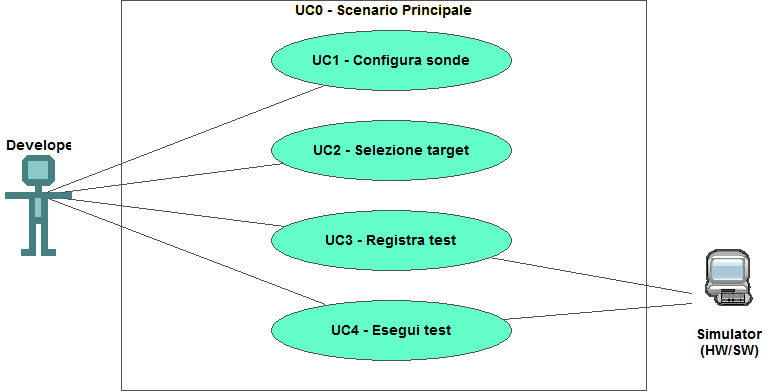
\includegraphics[width=0.9\columnwidth]{usecase/scenario-principale} 
%    \caption{Use Case - UC0: Scenario principale}
%\end{figure}

\section{Costruzione container tramite automazione: HDA Sandbox Builder}
%FLOW CHART ESECUZIONE batch file.